\documentclass[dvipsnames] {beamer}
\usepackage{cmlgc}
\usepackage{comment}
\usepackage{tikz}
\usefonttheme{serif}     % Font theme: serif
\usepackage[T2A]{fontenc}
\usepackage[utf8]{inputenc}
\usepackage[english]{babel}
\usepackage{amssymb,amsfonts,amsmath,mathtext,cite,enumerate,float} %подключаем нужные пакеты расширений
% \usepackage{cyrillic}
\usepackage{color, colortbl}
\usepackage{multirow}
\usepackage{graphicx}
\usepackage{graphics}
\usepackage{multirow}
\usepackage{url}
\usepackage{hyperref}
\usepackage{animate}
\usepackage{pifont}
\usepackage{wasysym}
\usepackage{marvosym}
\usepackage{appendixnumberbeamer} 
\usepackage{pgfpages}
\usepackage{systeme,mathtools}
\usepackage{mathtools}
\usepackage{listings}
\usepackage{xcolor} % for setting colors
\usepackage{mhchem}


\usepackage{ragged2e} %выравнивание текста по ширине слайда (\justifying)
%\setbeamercolor{background canvas}{bg=violet}

\usetheme{Madrid}
%\usecolortheme{crane}

%=================================================

\defbeamertemplate*{footline}{mytheme}{%
  \leavevmode%
  \hbox{%
    \begin{beamercolorbox}[wd=.2\paperwidth,ht=3ex,dp=1ex,center]{author in head/foot}%
      \usebeamerfont{author in head/foot}\insertshortauthor
    \end{beamercolorbox}%
    \begin{beamercolorbox}[wd=.7\paperwidth,ht=3ex,dp=1ex,center]{title in head/foot}%
      \usebeamerfont{title in head/foot}\insertshorttitle
    \end{beamercolorbox}%
    \begin{beamercolorbox}[wd=.1\paperwidth,ht=3ex,dp=1ex,right]{date in head/foot}%
      %\usebeamerfont{date in head/foot}\insertshortdate{}\hspace*{2em}
      %\insertframenumber{} / \inserttotalframenumber\hspace*{2ex} %номер текущего слайда / общее число слайдов
      \insertframenumber{} \hspace*{5ex}  %номер текущего слайда
  \end{beamercolorbox}}%
  \vskip0pt%
}
\usebeamertemplate{mytheme}
\beamertemplatenavigationsymbolsempty

\defbeamertemplate*{frametitle}{boldTitle}{%
  \begin{beamercolorbox}[wd=\paperwidth,ht=3ex,dp=3pt,center]{title in head/foot}%
    %        \ \textit{\textbf{\insertframetitle}} % курсивный заголовок слайда 
    \ \textbf{\insertframetitle}
  \end{beamercolorbox}
}
\usebeamertemplate{boldTitle}
\setbeamercovered{dynamic}

\setbeameroption{hide notes} % Only slides
%\setbeameroption{show only notes} % Only notes
%\setbeameroption{show notes on second screen=right} % Both
%\setbeamertemplate{note page}[plain]


%=================================================
% \titlegraphic{\includegraphics[width=\textwidth]{logo_conf.png}}

\addtobeamertemplate{title page}{\centering \includegraphics[scale=0.25]{all_emblems_in_one_file.png}}{}
\addtobeamertemplate{title page}{\centering \includegraphics[scale=0.05]{vnksf_logo1.png}}{}
\addtobeamertemplate{title page}{\centering \includegraphics[scale=0.17]{vnksf_logo.jpg}}{}
\date{\bf \footnotesize ЛФВЭ  им. Векслера и Балдина, ОИЯИ, Дубна}
\title[\bf ВНКСФ-26, Уфа, Магнитогорск]{\textbf{\large {Зачем мы ускоряем частицы? Ускорительный комплекс NICA как средство достижения цели}}}

\author[\bf П. Батюк]{\textbf{{\footnotesize П. Батюк, pavel.batyuk@jinr.ru}}} 
\institute{\bf \color{red} Всероссийская научная конференция студентов-физиков и молодых учёных (ВНКСФ-26)}

% \newpage \footnotesize April 14, 2016}}

\lstset{
  %    frame=tb, % draw a frame at the top and bottom of the code block
  tabsize=4, % tab space width
  showstringspaces=false, % don't mark spaces in strings
  %   numbers=left, % display line numbers on the left
  commentstyle=\color{blue}, % comment color
  keywordstyle=\color{blue}, % keyword color
  stringstyle=\color{red} % string color
}

\graphicspath{{../common_figures/}}

\begin{document}
\maketitle



\begin{frame}

\end{frame}

\begin{frame}
  \frametitle{\bf \centering Немного философии ...}
  \vskip -.75cm
  \begin{columns}[t]
    \column{.49\textwidth}
    \begin{figure}[H]
       \includegraphics[width=1.\linewidth]{1_53eb33689b80753eb33689b844.jpg}
    \end{figure}
    \begin{block}{}
      \bf \centering {\color{red} А зачем нужны ускорители?} \\
        {\color{blue} А зачем нам сталкивать частицы?} \\
        {\color{ForestGreen} А какие новые знания мы получим?} \\
        {\color{Magenta} Каковы возможные риски?}
    \end{block}
    \column{.49\textwidth}
    \begin{figure}[H]
       \includegraphics[width=1.\linewidth]{accel1.png}
    \end{figure}
    \vskip -.25cm
     \begin{figure}[H]
       \includegraphics[width=1.\linewidth]{accel2.png}
 \end{figure}
  \end{columns}
\end{frame}

\begin{frame}
  \bf
  \frametitle{\bf \centering Материя, которая нас окружает}
  \vskip -.75cm
  \begin{columns}[t]
    \column{.31\textwidth}
    \begin{block}{\bf \centering Микромир}
      Область предельно малых и непосредственно ненаблюдаемых материальных объектов
      \begin{figure}[H]
         \includegraphics[width=1.\linewidth]{atomStruct.jpg}
      \end{figure}
    \end{block}
    \column{.31\textwidth}
    \begin{block}{\bf \centering Макромир}
      \footnotesize Мир материальных объектов, соизмеримых по своим масштабам с человеком и его физическими параметрами
       \begin{figure}[H]
         \includegraphics[width=1.\linewidth]{9b2ad25ca7ee133edc66ae1202bcd4c2.jpg}
      \end{figure}
    \end{block}
     \column{.31\textwidth}
     \begin{block}{\bf \centering Мегамир}
       Сфера огромных космических масштабов и скоростей
       \begin{figure}[H]
         \includegraphics[width=1.\linewidth]{galaxy_photo.png}
       \end{figure}
     \end{block}
  \end{columns}
  \begin{block}{}
    \bf \centering \color{red} Ускоритель является идеальным инструментом для изучения материи на предельно малых масштабах
  \end{block}
  \note{Необходимость использования ускорителей для исследования структуры микромира очевидна. Во-первых, атомные ядра и элементарные частицы
    занимают очень малые области пространства, и проникновение в эти области требует высокой разрешающей способности зондирующего пучка,
    обеспечивающей взаимодействие отдельной пробной частицы с отдельным микрообъектом. Во-вторых, чем меньше микрообъект, тем он прочнее и проведение
    экспериментов с перестройкой или разрушением внутренней структуры такого объекта также требует большей энергии.}
\end{frame}

\begin{frame}
  \bf
   \vskip -.5cm
  \frametitle{\bf \centering Элементарные частицы}
  \begin{block}{}
    \begin{figure}[H]
      \includegraphics[width=1.\linewidth]{800px-Particle_overview-ru.png}
    \end{figure}
   
    \begin{center}
       \vskip -.3cm
      \color{red} Адроны (Л. Б. Окунь, 1962) и лептоны образуют вещество! \\
      \color{blue} Калибровочные бозоны - это кванты разных типов взаимодействий
    \end{center}
  \end{block}
\end{frame}

\begin{frame}
  
\end{frame}

\begin{frame}
  \frametitle{\bf \centering История Вселенной}
   \begin{figure}[H]
     \includegraphics[width=1.\linewidth]{CMB_Timeline300_no_WMAP_ru.jpg}
    \end{figure}
\end{frame}

\begin{frame}
  \bf
  \frametitle{\bf \centering История Вселенной}
   \begin{figure}[H]
     \includegraphics[width=1.\linewidth]{History_of_the_Universe-ru.png}
   \end{figure}
   \begin{block}{}
     \color{red} Понимание процессов в ранней Вселенной дают данные с ускорителей частиц.
     \color{blue} В настоящее время нет ни существующих, ни планируемых ускорителей, которые позволят получить энергии порядка Планковской энергии.
   \end{block}
\end{frame}

\begin{frame}
  
\end{frame}

\begin{frame}
  \bf
  \frametitle{\bf \centering Ускорители заряженных частиц}
  \vskip -.25cm
  \begin{block}{}
    \footnotesize Формирование пучка частиц с требуемыми для эксперимента характеристиками (энергия, поток, интенсивность, пространственные размеры)
  \end{block}
  \vskip -.7cm
  \begin{columns}[t]
    \column{.49\textwidth}
    \begin{block}{}
      \begin{figure}[H]
        \includegraphics[width=1.\linewidth]{fa01.png}
      \end{figure}
    \end{block}

    \column{.49\textwidth}
    \begin{block}{\bf \centering Траектория}
      \begin{itemize}
      \item Линейные
      \item Циклические
      \end{itemize}
    \end{block}
    \begin{block}{\bf \centering Типы частиц}
      \begin{itemize}
      \item Электроны и протоны
      \item Ионы, в том числе и тяжёлые (свинец)
      \end{itemize}
    \end{block}
  \end{columns}
  \vskip -.2cm
  \begin{block}{}
    \footnotesize Рождение новых частиц происходит в результате преобразования кинетических энергий взаимодействующих (сталкивающихся) частиц.
    \color{red} Чем больше масса частицы, которую необходимо получить в столкновении, тем больше должна быть энергия сталкивающихся частиц.
  \end{block}
  \note{Любой ускоритель конструктивно состоит из трёх частей (см. рисунок) – системы, где “изготавливаются” ускоряемые частицы (инжектор),
    ускорительной системы, где низкоэнергичные частицы от инжектора (обычно сформированные в виде локализованных в пространстве сгустков) увеличивают
    энергию до проектной, и системы транспортировки (вывода) пучка к экспериментальной установке.}
\end{frame}

\begin{frame}
  \bf
  \frametitle{\bf \centering Преимущества и принцип работы коллайдера}
  \vskip -.75cm
  \begin{columns}[t]
    \column{.49\textwidth}
    \begin{block}{}
      \begin{figure}[H]
        \includegraphics[width=1.\linewidth]{fa07.png}
      \end{figure}
    \end{block}
     \begin{block}{\bf \centering \footnotesize Два сталкивающихся сгустка частиц (банча) в коллайдере:}
      \begin{figure}[H]
        \includegraphics[width=1.\linewidth]{fa08.png}
      \end{figure}  
    \end{block}

    \column{.49\textwidth}
    \begin{block}{}
      {\scriptsize
      \begin{itemize}
      \item Во встречных пучках, двигающихся навстречу друг другу, накапливается максимально возможное число частиц (до $10^{15}$ в пучке).
      \item Огромная разница между кинетическими энергиями в ускорителе с неподвижной мишенью и со встречными пучками.
      %\item Встречные пучки состоят из отдельных сгустков частиц, называемых банчами (от англ. bunch), двигающихся с определенным интервалом (частотой) друг
      %  за другом.       
      \end{itemize}
      }
    \end{block}
    \begin{block}{\bf \centering Светимость:}
      \begin{equation*}
        N = f \dfrac{n_{1} n_{2}}{S} \sigma
      \end{equation*}
      \begin{equation*}
        L = f \dfrac{n_{1} n_{2}}{S}
      \end{equation*}
      \footnotesize N - число актов реакции \\
      \footnotesize $n_{1, 2}$ - концентрации частиц в сгустке \\
      \footnotesize f - частота столкновений
    \end{block}    
  \end{columns} 
\end{frame}

\begin{frame}
  
\end{frame}

\begin{frame}
  \vskip -.3cm
  \frametitle{\bf \centering Эволюция столкновения по времени}
   \begin{block}{}
    \begin{figure}[H]
      \includegraphics[width=1.\linewidth]{qgp.jpg}
    \end{figure}
  \end{block}
\end{frame}

\begin{frame}
  
\end{frame}


\begin{frame}
  \bf
  \frametitle{\bf \centering Действующие адронные коллайдеры}
  \vskip -.8cm
  \begin{columns}[t]
    \column{.49\textwidth}
    \begin{block}{\bf \centering Релятивистский коллайдер тяжёлых ионов (RHIC)}
      \begin{figure}[H]
       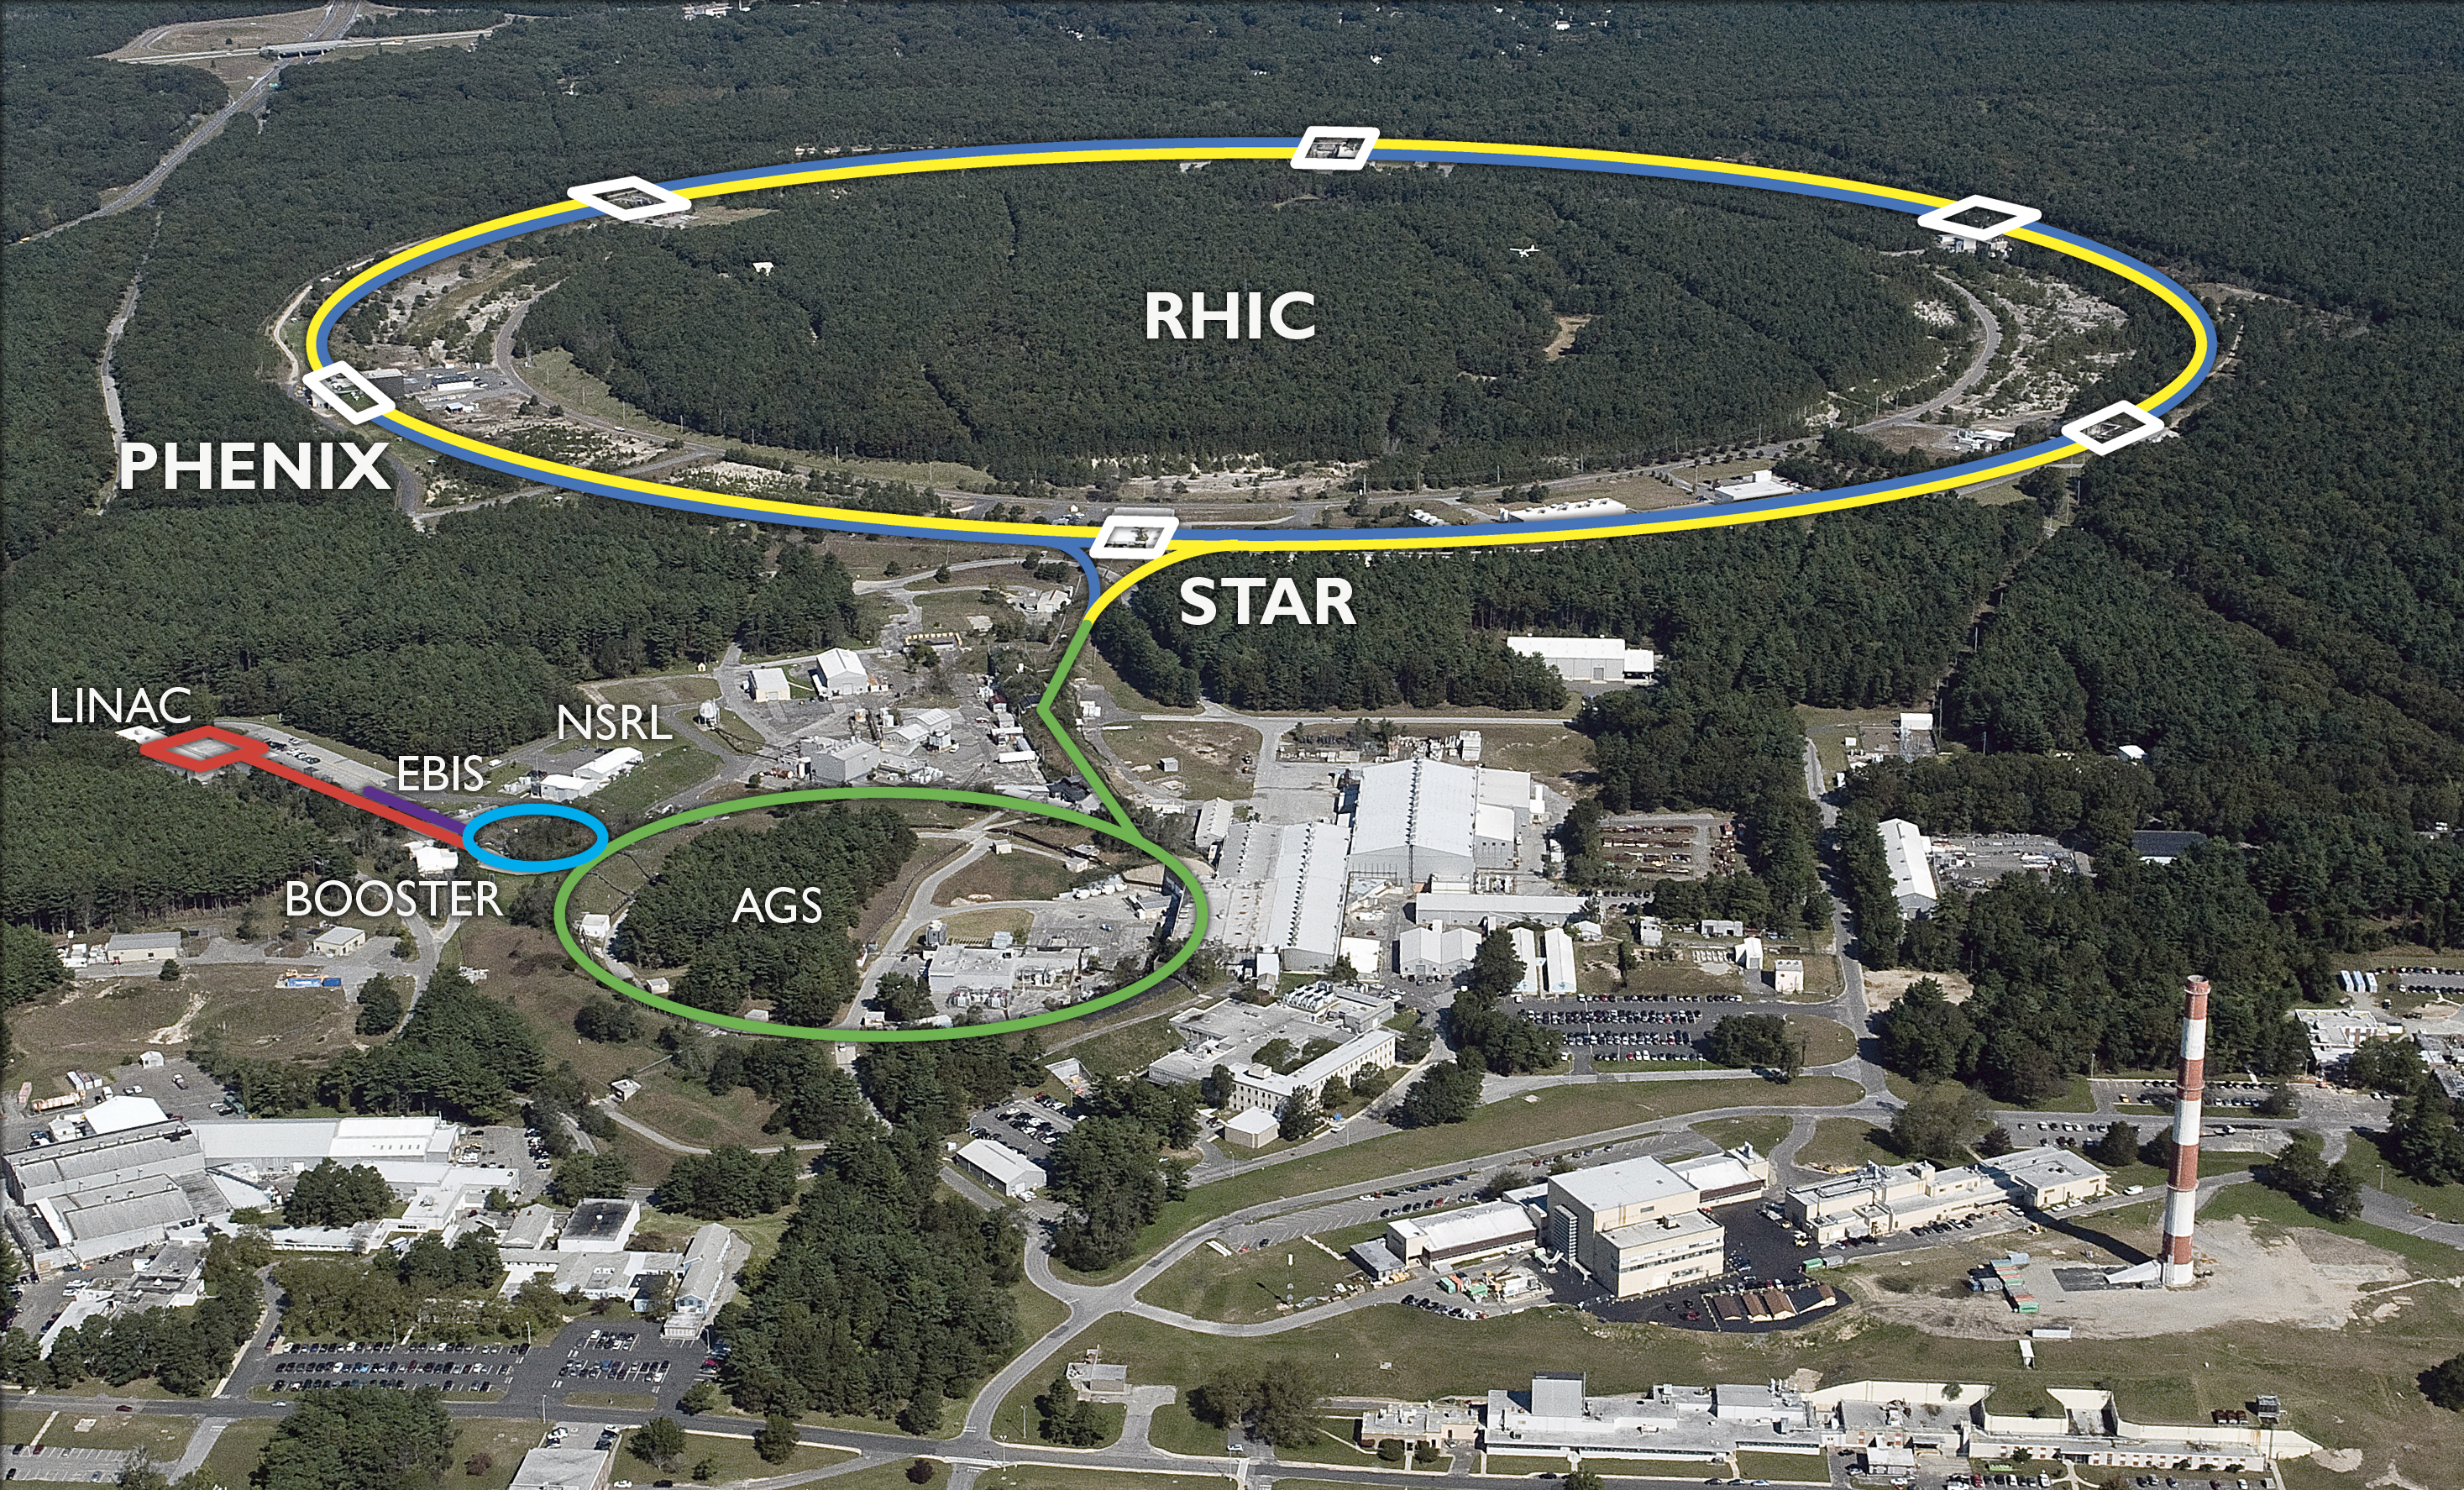
\includegraphics[width=1.\linewidth]{7979381212_c604577389_o.jpg}
      \end{figure}
      \vskip -.6cm
      \begin{itemize}
      \item США, Брукхейвенская национальная лаборатория
      \item Периметр $\sim$ 4 км
      \item pp, AuAu, CuCu, dAu, до 200 {\color{red} ГэВ/нуклон} 
      \end{itemize}
    \end{block}
    \column{.46\textwidth}
    \begin{block}{\bf \centering Большой адронный коллайдер (LHC)}
       \begin{figure}[H]
       \includegraphics[width=1.\linewidth]{lhc-ring-aerial_2.jpg}
       \end{figure}
        \vskip -.6cm
      \begin{itemize}
      \item Швейцария-Франция, ЦЕРН
      \item Периметр $\sim$ 27 км
      \item pp (до {\color{blue} 7 ТэВ}), pPb, PbPb (до {\color{blue} 2.76 ТэВ/нуклон}) 
      \end{itemize}
    \end{block}
  \end{columns}
\end{frame}




\begin{frame}
  \frametitle{\bf \centering Зачем нам нужен третий адронный коллайдер?}

\end{frame}


\begin{frame}
  \frametitle{\bf \centering Комплекс NICA}
   \begin{block}{}
     \begin{figure}[H]
       \includegraphics[width=1.\linewidth]{NICA_complex-ru.png}
     \end{figure}
   \end{block}

\end{frame}


\begin{frame}
  \bf
  \begin{center}
    \Huge{Немного дополнительной информации об ОИЯИ}
  \end{center}
\end{frame}

\begin{frame}
   \bf
   \vskip -.3cm
   \begin{block}{}
     \begin{figure}[H]
       \includegraphics[width=1.\linewidth]{Screenshot_20200311_150621.png}
     \end{figure}
   \end{block}
   \vskip -.85cm
   \begin{columns}[t]
     \column{.49\textwidth}
     \begin{block}{}
       \begin{itemize}
       \item \color{blue} 7 Лабораторий в составе Института: ЛЯП, ЛТФ, ЛИТ, ЛРБ, ЛНФ, ЛЯР, ЛФВЭ
       \end{itemize}
     \end{block}
     \column{.49\textwidth}
     \begin{block}{}
       \begin{itemize}
       \item \color{red} 18 стран-участниц
       \item \color{ForestGreen} Обширная образовательная деятельность
       \end{itemize}
     \end{block}
   \end{columns}
\end{frame}

\begin{frame}
  

\end{frame}

\begin{frame}
  \bf
  \vskip -.75cm
  \begin{columns}[t]
    \column{.1\textwidth}
     \column{.8\textwidth}
  \begin{block}{}
    \begin{figure}[H]
      \includegraphics[width=1.\linewidth]{Screenshot_20200311_145224.png}
    \end{figure}
  \end{block}
  
 \column{.1\textwidth}
  \end{columns}
   \begin{columns}[c]
    \column{.6\textwidth}
    \vskip -.4cm
    \begin{block}{}
       \vskip -.1cm
    {\footnotesize 
      \begin{itemize}
      \item Приём студентов в ОИЯИ
      \item Студенческие практики
      \item Подготовка квалификационных работ
      \item Школы и конференции
      \item Инженерный практикум
      \item {\color{red} Групповые экскурсии для студентов}
      \end{itemize}
      }
  \end{block}
    \column{.39\textwidth}
    \vskip -.3cm
    \begin{block}{}
      \begin{figure}[H]
        \includegraphics[width=1.\linewidth]{Screenshot_20200311_145707.png}
        Более подробно:
        \url{http://uc.jinr.ru}
    \end{figure}
    \end{block}
  \end{columns}
\end{frame}



\begin{frame}

\end{frame}


\begin{frame}
  \bf
  \vskip -.3cm
  \begin{block}{}
    \begin{figure}[H]
      \includegraphics[width=1.\linewidth]{Screenshot_20200311_142200.png}
    \end{figure}
  \end{block}
  \begin{columns}[c]
    \column{.6\textwidth}
    \vskip -.4cm
    \begin{block}{}
       \vskip -.1cm
    {\scriptsize 
      \begin{itemize}
      \item Теоретическая  и математическая физика
      \item Физика элементарных частиц (в т.ч. {\color{red} NICA})
      \item Нейтронная физика
      \item Физика конденсированных сред
      \item Радиобиологические исследования
      \item Сети, компьютинг, вычислительная физика
      \item Ускорительная физика и техника
      \item Детекторы частиц
      \item Прикладные исследования с применением методов ядерной физики
      \end{itemize}
      }
  \end{block}
    \column{.39\textwidth}
    \vskip -.3cm
    \begin{block}{}
      \begin{figure}[H]
        \includegraphics[width=1.\linewidth]{Nuclotron.jpg}
        Более подробно:
        \url{http://students.jinr.ru}
    \end{figure}
    \end{block}
  \end{columns}
\end{frame}


\begin{frame}
  \begin{center}
    \Huge{\bf \centering Спасибо за внимание! \\
      $$ $$ \\
    Ваше желание присоединиться к нашему коллективу очень приветствуется!}
  \end{center}
\end{frame}



\end{document}
